\chapter{Results}
\begin{toDo}
	\section{Architecture}
	Come accennato nei capitoli precedenti, il sistema di analisi delle immagini richiede di confrontare l'opera sconosciuta con quelle note.

	\noindent L'immagine viene preprocessata rimuovendo elementi inquinanti che non riguardano la grafia, lasciando essenzialmente un'immagine in scala di grigi con la grafia dell'autore in tonalità scura e lo sfondo bianco. Inoltre, il tratto dell'autore potrebbe necessitare di uno spessore specifico rispetto ai caratteri impressi e la risoluzione (espressa in \gls{ppi}) deve essere conforme al dataset.

	\noindent L'immagine così preprocessata sarà quindi sintetizzata: un programma ne estrae tutte le tessere con una dimensione specifica conforme al dataset. In seguito, l'immagine sarà confrontata con ogni immagine del dataset (o con le più rappresentative per ogni autore).

	\noindent In questo capitolo si effettueranno analisi di ogni passaggio illustrato in questa tesi al fine di vedere come ogni singola componente agisce sulle immagini esaminate. Non solo, si mostreranno anche le analisi effettuate per stabilire specifiche decisioni e parametri usati durante la fase di progettazione.

	\bigskip\noindent La costruzione del dataset avviene con un procedimento lievemente diverso. Ogni immagine di cui l'autore è noto viene confrontata completamente con tutte le altre già note. Essendo il comparison value simmetrico, sarà sufficiente esaminare la metà di tutti i confronti possibili. Se si è in possesso di $n$ immagini, pensiamo di voler riempire una tabella quadrata $n\times n$ con valori reali. Assumendo comparison value $0$ tra immagini con se stesse, si può concludere che in totale saranno richiesti $\frac{n^2-n}{2}$ confronti.

	\noindent Per questa ragione, l'algoritmo per ogni riga esaminerà la metà dei possibili confronti come mostrato in \cref{fig:distance_computation}. In particolare, se $n$ è dispari, per ogni riga si faranno $\frac{n-1}{2}$ confronti (e altrettanti saranno memorizzati per via della simmetria), mentre se $n$ è pari, allora $\frac{n}{2}$ confronti saranno effettuati se la riga $i$ è pari (la prima riga ha indice $0$) e $\frac{n}{2}-1$ se la riga $i$ è dispari. Questa procedura permette una analisi più uniforme ed efficiente per numerosi dati, specie se accompagnata da shuffle per riga e per colonna.

	\begin{figure}[H]
		\centering
		\includegraphics[width=0.7\linewidth]{Figures/analysis_sort.png}
		\caption[Visit all couples]{The algorithm for each row computes half of all components. In the image, the algorithm follows the order of the numbers and alternately takes the cells such that the lower diagonal is not directly computed and the upper diagonal is directly computed. For example, in the $3^\text{-th}$ row, the algorithm computes directly the first column (number $5$ in cyan) and the next-to-last column (number $6$ in cyan), while the second column is already computed (number $3$ in green square) and the last column is not yet computed.}
		\label{fig:distance_computation}
	\end{figure}

	\subsection{Challenges}
	L'implementazione del codice ha richiesto notevoli sforzi poiché gran parte dei framework richiesti non erano esistenti, inoltre le limitazioni della potenza di calcolo e il tempo a disposizione hanno rappresentato un forte vincolo. Questo ha richiesto la stesura di codice altamente prestante e sofisticato per ottimizzare l'efficienza computazionale.

	\noindent In generale, il progetto ha richiesto largo uso di \gls{Python} e \gls{CUDA}. Durante la sua realizzazione si sono utilizzati software specifici per debugging, logging e testing, utili per monitorare il corretto funzionamento del software. Sono stati impiegati strumenti di documentazione automatica e gestione delle versioni del codice. Inoltre, è stato adottato un robusto sistema di gestione degli errori e delle sessioni di calcolo, con meccanismi di backup (detti "checkpoint") per scongiurare la perdita di dati preziosi. Il software utilizza anche file temporanei per aumentare la capacità di memorizzazione oltre i limiti della memoria principale.

	\noindent Per queste ragioni, il codice (composto da un totale di $3480$ righe) è difficilmente riportabile per intero in questo testo ed è consultabile nella repository \gls{github}:\\ \url{https://github.com/StefanoMagriniAlunno/MMATH_thesis}.

	\bigskip\noindent La macchina che ha prodotto i risultati illustrati in questo capitolo ha le seguenti specifiche tecniche:
	\texttt{\begin{itemize}
		\item \textbf{processor}: 11th Gen Intel(R) Core(TM) i7-11370H @ 3.30GHz
		\begin{itemize}
			\item[-] Cores: 4
			\item[-] Thread(s) per core: 2
			\item[-] CPU max MHz: 4800
			\item[-] Caches:
			\begin{itemize}
				\item[*] L1d 192KiB (4 instances)
				\item[*] L1i 128KiB (4 instances)
				\item[*] L2 5MiB (4 instances)
				\item[*] L3 12MiB (1 instances)
			\end{itemize}
		\end{itemize}
		\item \textbf{memory}: 16 GiB
		\begin{itemize}
			\item[-] SODIMM DDR4 Synchronous 3200 MHz (0,3 ns)
			\item[-] SODIMM DDR4 Synchronous 3200 MHz (0,3 ns)
		\end{itemize}
		\item \textbf{memory}: 16 GiB
		\begin{itemize}
			\item[-] SODIMM DDR4 Synchronous 3200 MHz (0,3 ns)
			\item[-] SODIMM DDR4 Synchronous 3200 MHz (0,3 ns)
		\end{itemize}
		\item \textbf{graphic processor unit}: NVIDIA GeForce GTX 1650
		\begin{itemize}
			\item[-] Cores: 896
			\item[-] stream multiprocessor: 14
			\item[-] VRAM: GDDR5 4096 MiB
			\item[-] CUDA capability: 7.5
		\end{itemize}
	\end{itemize}}
	\noindent Saranno visionate anche le prestazioni per sottolineare come l'uso di processori grafici possa essere estremamente utile per questo tipo di fini.

	\bigskip\noindent Il codice fa uso di wrapping, ossia di programmi in grado di far scorrere il flusso di uno script di \gls{Python} in un codice precompilato di \gls{cxx}. In questo modo si è realizzato con codice \gls{Python} uno script di avvio per le sessioni di calcolo che prepara file e report utili, recupera specifiche hardware e configurazioni del calcolo da eseguire. Laddove è richiesto un'intensivo calcolo lo script \gls{Python} chiamerà una libreria precompilata scritta in \gls{cxx}. In questo modo il codice \gls{cxx} potrà essere più essenziale e quindi leggibile.

	\noindent Per fare un esempio di avvio di una comparazione tra opere, lo script principale di \gls{Python} si occupa di preparare il sistema operativo, convalidare i parametri usati ed eventuali checkpoint. Quindi, fornisce tutti gli input richiesti al wrapper (scritto in \gls{cxx}) il quale convalida eventuali errori di sintassi e traduce i tipi di valori di \gls{Python} in tipi comprensibili al \gls{cxx}. Di seguito, questi valori vengono passati ad uno starter che prepara un logger e legge eventuali file inizializzando di fatto la memoria principale. Il programma scritto in \gls{cxx} chiama il programma scritto in \gls{CUDA} il quale si occupa di leggere i dettagli tecnici della \gls{gpu} (usando apposite librerie) per configurare un piano di calcolo che massimizza le prestazioni e che sia robusto. Infine, verranno comunicate le istruzioni alla \gls{gpu} come kernel (codice esplicito che compilerà la \gls{gpu} stessa in runtime). Poiché la memoria della \gls{gpu} è limitata, è importante far attenzione che i dati siano passati parzialmente e usare la memoria principale come appoggio.

	\noindent I dati ottenuti dalla \gls{gpu} vengono passati alla funzione chiamante in \gls{cxx} la quale li memorizza in modo opportuno e restituisce il controllo allo script di \gls{Python} chiamante. In caso di errori tutto viene documentato e riportato al chiamante per gestirli in modo opportuno.

	\noindent Questo tipo di strategie per realizzare codice prestante sono tipiche nelle librerie di calcolo scientifico che spesso mostrano una funzione principale chiamante e funzioni compilate nascoste, un esempio è CuPy, una libreria \gls{Python} la quale installazione prevede anche la compilazione.

    \section{Pre processing}
    Il pre processing è una fase importante del confronto tra opere ignote con il dataset. In particolare si preoccupa di far rispettare delle specifiche qualitative dell'immagine per lo più soggettive, non è quindi detto che si faccia uso dello stesso algoritmo per ogni immagine. Il fine ultimo è eliminare dati evidentemente inquinanti per far rispettare un certo standard e presentare l'immagine al software nel giusto modo. Essenzialmente si avvicina il dato reale al dato ideale ammissibile teoricamente dal software.

    \noindent Come già illustrato in \cref{alg:CleaningFFT}, il preprocessing adottato per i dati raccolti fa uso principalmente di una compressione con \gls{fft}. In questa sezione saranno illustrati i risultati passo passo seguendo l'algoritmo.

    \paragraph{FFT}
    Il primo step dell'algoritmo di preprocessing è applicare \gls{fft} all'immagine normalizzata, quindi con pixel grigi aventi valori di media $0$ e varianza $1$. Come osservato, attraverso immagini sintetiche, i quadretti nello sfondo delle pagine di appunti sono pattern ricorrenti che tipicamente non sono propri della scrittura di un testo. Questa ricorrenza è meglio visibile attraverso l'uso di trasformate di Fourier.

   	\noindent In \cref{fig:fft_application} è visibile il pattern dei quadretti come frequenze alte separatamente su $x$ e su $y$ di significiativa intensità.

    \begin{figure}[H]
    	\centering
    	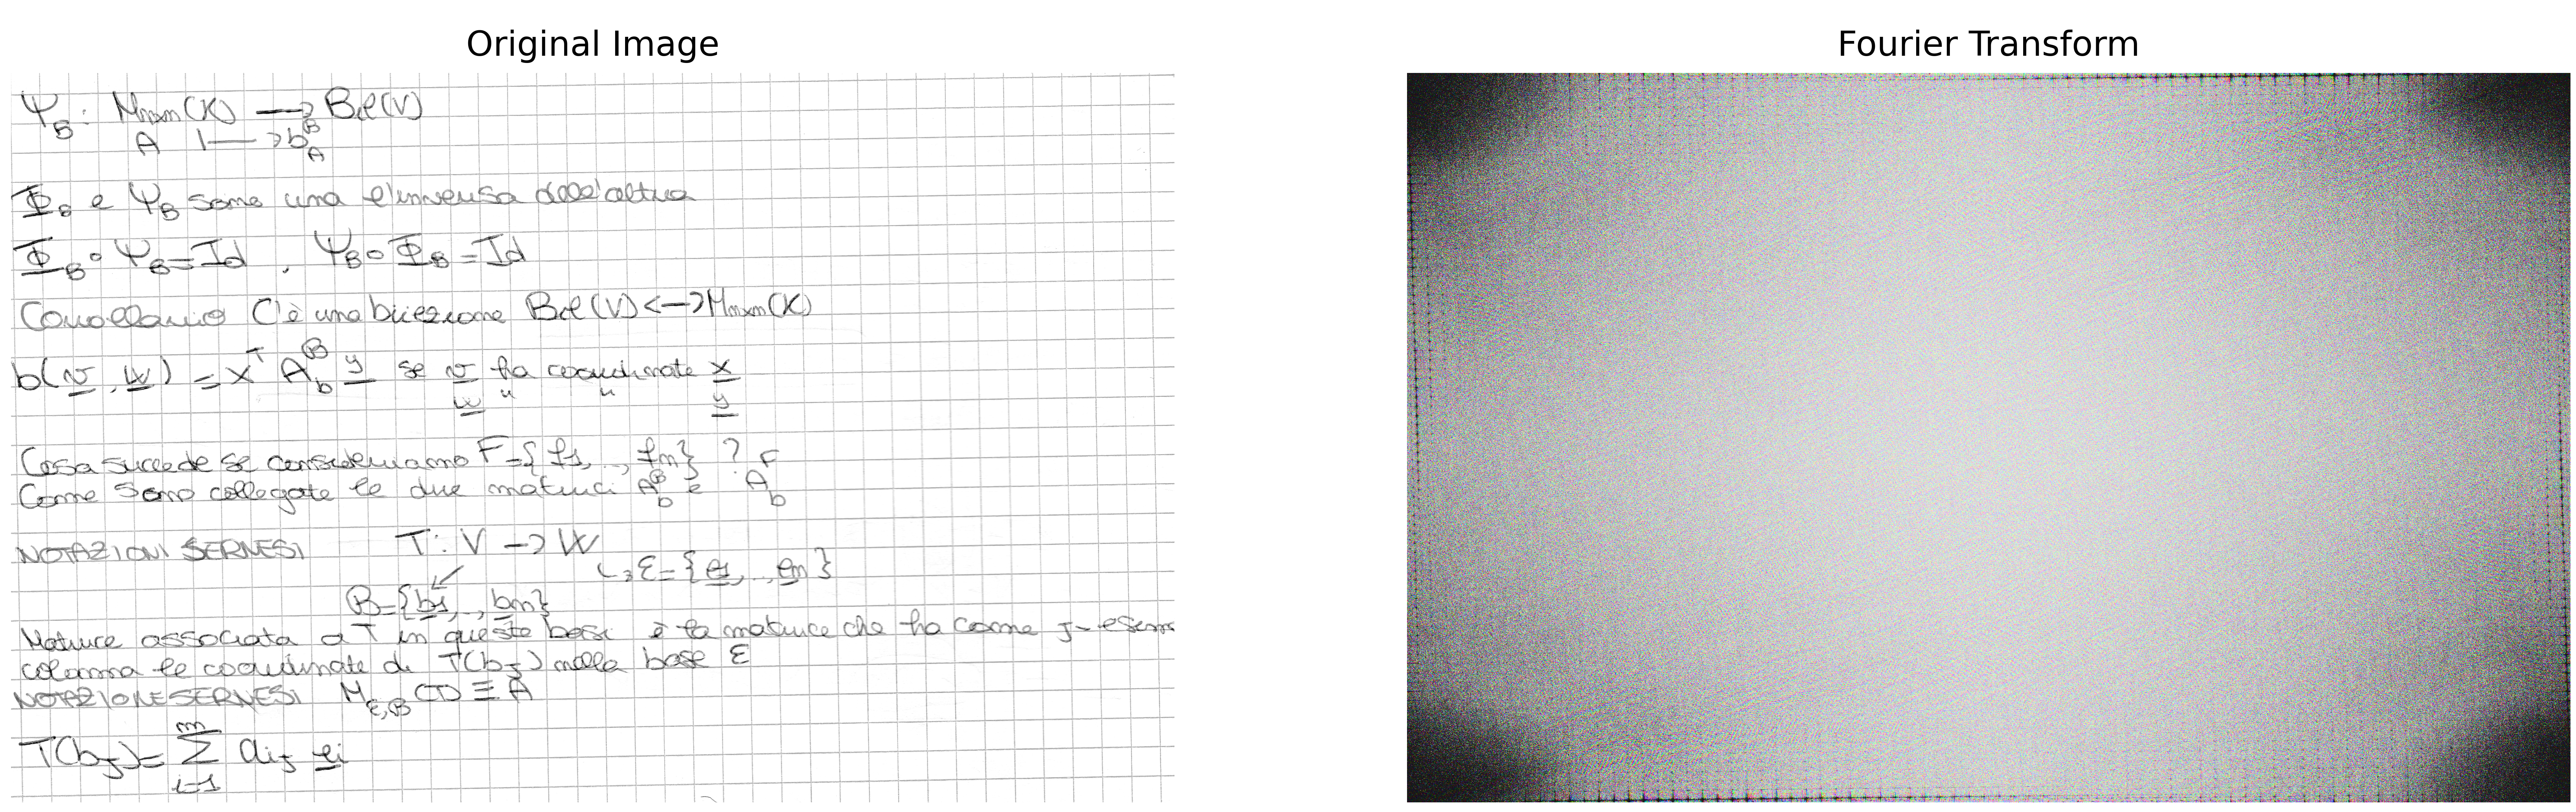
\includegraphics[width=1.0\linewidth]{Figures/fft_application.png}
    	\caption[fft application]{We can observe significant frequencies along the edge of the second image.}
    	\label{fig:fft_application}
    \end{figure}

	\noindent Il programma rimuove il $p$-percentile delle frequenze con più alta ampiezza. Dopodiché ricostruisce l'immagine originale usando le frequenze rimaste, cui ampiezza non è stata annullata. In \cref{fig:fft_percentile} si vedono varie ricostruzioni usando differenti percentili e una normalizzazione tra $0,1$ dei grigi ottenuti. Osserviamo come $p=0.1\%$ è una scelta appropriata da cui cominciare le analisi.

	\begin{figure}[H]
		\centering
		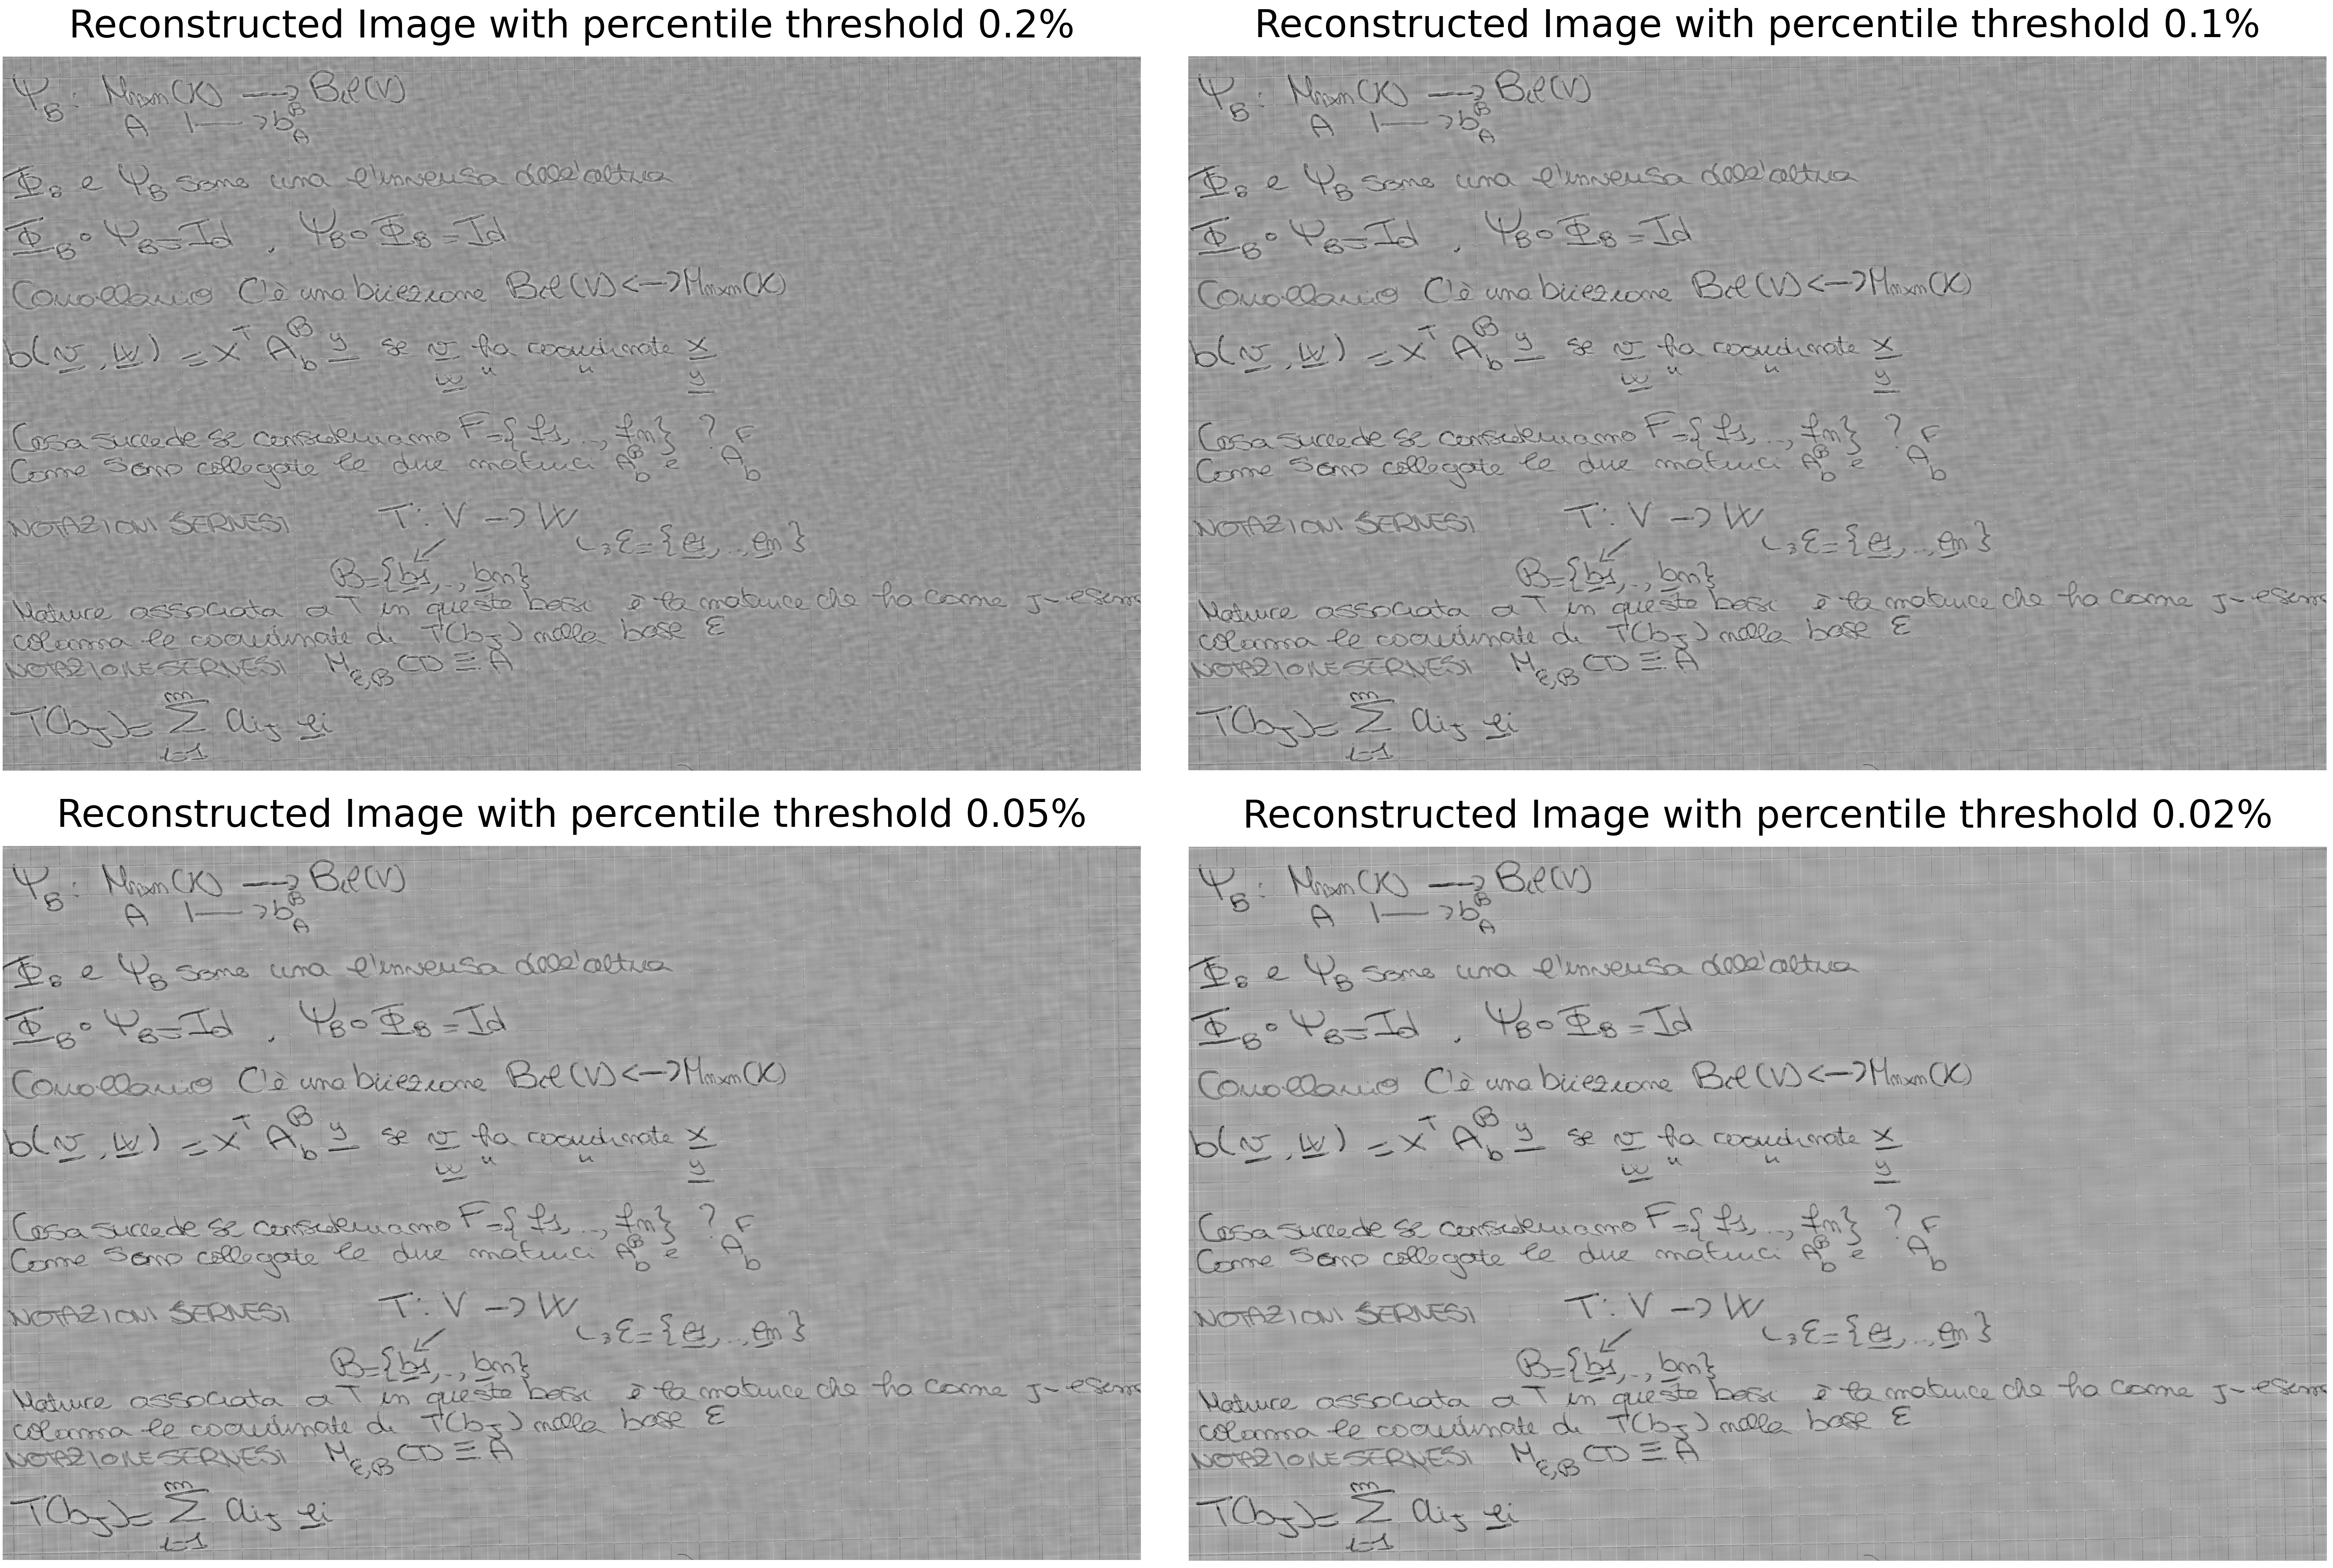
\includegraphics[width=1.0\linewidth]{Figures/fft_percentile.png}
		\caption[comparing different percentiles in fft]{Si può osservare che un percentile tra $0.1\%$ e $0.05\%$ è un buon compromesso, i quadretti sembrano sparire e la scrittura rimane intaccata.}
		\label{fig:fft_percentile}
	\end{figure}

	\noindent Si può osservare che la normalizzazione effettuata per visualizzare queste immagini nasconde il fatto che i pixel sono in realtà tutti visibilmente uguali tra loro. L'idea quindi è individuare quanti pixel erano parte certamente dello sfondo bianco della pagina e quanti invece delle grafie. Analizzando le immagini originali si è osservato che i pixel con valore di grigio inferiore a $0.2$ sono certamente parte delle grafie, invece se il valore è superiore a $0.8$ sono certamente parte dello sfondo bianco della pagina. Quindi l'algoritmo recupera quanti pixel sono certamente delle grafie e quanti non lo sono. In figura \cref{fig:fft_diagrams} un'illustrazione di questa analisi.

	\begin{figure}[H]
		\centering
		\includegraphics[width=0.8\linewidth]{Figures/fft_diagrams.png}
		\caption[different density after fft compression]{Nell'immagine originale si osserva che la densità dei grigi presentava, per ovvie ragioni, molti pixel bianchi. Mentre nell'immagine ricostruita sono per lo più grigi medi. Per mantenere una distribuzione quanto meno simile a quella di partenza bisogna separare di più i colori tra loro. Per questa ragione si contano nell'immagine originale quanti pixel avevano un livello grigio superiore a $0.8$ (linea verde) che ne certifichi l'appartenenza allo sfondo, così anche per la quantità di pixel sufficientemente scuri da considerarsi parte delle grafie (con un livello di grigio inferiore a $0.2$, linea rossa). Così nell'immagine ricostruita è ragionevole assumere che i pixel più chiari siano parte dello sfondo e i pixel più scuri siano parte delle grafie, identificando così $2$ threshold per l'immagine ricostruita.}
		\label{fig:fft_diagrams}
	\end{figure}

	\noindent Quindi l'algoritmo identifica un livello di grigio $\texttt{h}_\texttt{up}$ nell'immagine ricostruita sopra il quale il numero di pixel è uguale (o poco inferiore) al numero di pixel considerati parte dello sfondo nell'immagine originale. Similmente per $\texttt{h}_\texttt{down}$, sotto il quale i pixel ricostruiti sono così scuri che risulta ragionevole pensare che facciano parte delle grafie.

	\noindent Noti i due estremi nell'immagine ricostruita, si esegue una trasformazione lineare dei livelli di pixel che fa sì che gli estremi abbiano livelli rispettivamente $0$, $1$:
	\[
		\texttt{gray}_\texttt{new} = \frac{\texttt{gray}_\texttt{old} - \texttt{h}_\texttt{down}}{\texttt{h}_\texttt{up} - \texttt{h}_\texttt{down}}
	\]
	Di conseguenza i pixel con un livello inferiore a $0$ o superiore a $1$ saranno resi automaticamente $0$, $1$, rispettivamente, usando la trasformazione \texttt{clamp}.

	\noindent In \cref{fig:fft_results} si mostrano i risultati di questo processo per percentili $0.1\%$ e $0.05\%$ su $2$ campioni. Come si osserva, il risultato non è molto differente ad occhio nudo. Per preservare meglio le grafie, a costo di lasciare più segni di quadretti, si è deciso di usare $p=0.05\%$. L'idea è sperare che questo rumore sia in qualche modo catturato dal clustering \gls{fcm}.

	\begin{figure}[H]
		\centering
		\includegraphics[width=1.0\linewidth]{Figures/fft_results.png}
		\caption[results of "fft cleaner"]{In figura sono mostrate due immagini preprocessate usando differenti percentili. La prima colonna fa uso di $p=0.05\%$, la seconda di $p=0.1\%$, ogni riga fa riferimento ad un'opera del dataset.}
		\label{fig:fft_results}
	\end{figure}

    \section{Synthesis}
    Una volta che le immagini sono state preprocessate e quindi rese conformi al dataset secondo parametri "umani", si procede con la sintesi che di fatto rende le opere conformi da un punto di vista oggettivo. In particolare le opere saranno ridefinite come un elenco (ordinato o meno) delle loro tessere che saranno quadrate e aventi la stessa forma.

    \noindent Come già accennato, lo script \gls{Python} si occupa di preparare il sistema operativo e ricavare velocemente input e parametri hardware per i programmi precompilati a più basso livello. In questo caso lo script \texttt{synthesis.py} in poche linee di codice crea le cartelle utili nelle quali un programma \gls{cxx} può memorizzare le sintesi ottenute con il seguente frame di codice:

\begin{lstlisting}[style=code, language=C, rulecolor=\color{blue}]
/** @brief In this code we use OpenMP API to realize an array with all tiles.
 *
 *  @param[in] byte_board : the array with all pixels
 *  @param[out] cells : the array with all tiles of the image
 *  @param n_threads : the number of used threads in the first loop
 *  @param height : the height of the image
 *  @param width : the width of the image
 *  @param n_tiles : the size of tiles
 *
 *  @details This code uses a bijective map from tiles and "short"image, i.e. an image with shape width_short, height_short. Each tiles will be assigned to its first pixel (up/sx).
 *  "omp parallel for" is a directive of OpenMP that executes a for cycle using more indipendent threads. In this case the schedule is "static" i.e. each thread knows in advance all its loops.
 */
unsigned width_short = width - n_tiles + 1,
         height_short = height - n_tiles + 1;
#pragma omp parallel for schedule(static) num_threads(n_threads)
for (unsigned row = 0; row < height_short; ++row)
for (unsigned col = 0; col < width_short; ++col)
  for (unsigned i = 0; i < n_tiles; ++i)
  for (unsigned j = 0; j < n_tiles; ++j) {
    long unsigned index_out = ((row * width_short + col) * n_tiles + i) * n_tiles + j; // [row-i, col-j, i,j]
    long unsigned index_in = (row + i) * width + col + j;
    cells[index_out] = byte_board[index_in];
    }\end{lstlisting}

    \noindent Usare più \gls{thread} per compiere un ciclo aiuta ad aumentare le prestazioni del ciclo di un fattore moltiplicativo. Inoltre l'accesso in scrittura in \texttt{cells} per \texttt{row} differente non rischia problemi di concorrenze, ossia più \gls{thread} che scrivono sulla medesima cella di memoria. Poi in questo caso il tempo di esecuzione nominale di un loop non dipende dalla scelta della riga, per questa ragione una schedule statica riduce di molto anche i tempi stessi per gestire il gruppo di thread generati.

    \noindent La tecnica del multi-threading si usa per ottimizzare i tempi di esecuzione di piccoli passaggi parallellizzabili. E' quindi inusuale vedere applicati questo tipo di tecniche ad alto livello, come ad esempio analizzare due immagini in contemporanea. Questo perché da un lato avviare più processi ad alto livello riduce i tempi totali di avvio, ma dall'altro aumenta la memoria richiesta, questo dipende molto dal problema che ci si pone di fronte.

    \noindent Poiché ogni immagine diventa un insieme di tessere, è chiaro che questa potrebbe occupare più spazio in memoria. Il numero di componenti dell'array \texttt{cells} sarà:\\ $(w-n+1)(h-n+1)n^2$, dove $w,h$ sono le dimensioni dell'immagine originale e $n$ il size delle tessere.\\
    Di conseguenza è difficile pensare di poter gestire molteplici thread ad alto livello.

    \subsection{A simple analysis}
    Poiché le sintesi sono un set di punti ad alta dimensione è difficile poterle visualizzare. Qui di seguito sarà proposta una visualizzazione "grossolana" che riduce la dimensionalità da $\mathbb{R}^{16}$, per tessere $4\times4$, a $\mathbb{R}^6$. Questa procedura consiste in una \gls{pca} e sarà visualizzato solo un sotto-campione di $\num{5000}$ tessere. Questa visualizzazione può essere mal interpretataa poiché si ha una forte perdita di dimensionalità e numerosità dei dati, quindi i grafici qui proposti sono solo a fine illustrativo.

    \noindent Come si può osservare in \cref{fig:synth_glbvisual} vi è una regione dove le tessere sono molto concentrate. L'ipotesi più ragionevole è che il background delle immagini produce molte tessere chiare che formano un cluster denso. Per confermare questa ipotesi si sono evidenziati questi punti con le tessere originali.

    \begin{figure}[H]
    	\centering
    	\includegraphics[width=0.8\linewidth]{Figures/synth_glbvisual.png}
    	\caption[global visualisation of a synthesis using PCA]{In figura è mostrato, con degli scatter di ugual dimensione, un campione di tessere raccolte da un'immagine. Usando i colori si possono riconoscere $6$ dimensioni. Come si può osservare, le tessere del background sono per lo più concentrate in $\vec{0}$. Mentre le tessere delle grafie sono più rarefatte.}
    	\label{fig:synth_glbvisual}
    \end{figure}

    \section{Comparison}
    Il confronto tra le distribuzioni definisce la dissimilarità tra opere, poiché questo processo ha un costo computazionale oneroso sarà importante studiare la relazione tra la qualità del risultato in confronto al tempo impiegato e i parametri scelti. In particolare si sta parlando di:
    \begin{itemize}
    	\item Ridurre il numero di iterazioni usate per il calcolo dei centroidi in \gls{fcm}.
    	\item Ridurre il numero di centroidi usati in \gls{fcm}.
    	\item Ridurre la dimensionalità con \gls{pca} prima di eseguire \gls{fcm}
    	\item Ridurre il numero di dati prima di eseguire \gls{fcm}
    \end{itemize}

	\subsection{Implementation}
	L'implementazione dell'algoritmo di comparazione è molto lunga e articolata, qui sarà mostrato solo uno schema generale. In particolare si vedrà come sono gestiti i dati attraverso la \gls{gpu} considerandone i limiti fisici.


	\noindent Visionando le formule di aggiornamento si può notare che è possibile usare degli update attraverso dei batch. In particolare i limiti fisici di memoria della \gls{gpu} non permettono di calcolare un update per intero ma sarà necessario cumulare calcoli parziali su dati parziali.

	\noindent Qui sono esplicitate le formule di aggiornamento teoriche:

	\begin{align*}
		C_{j}^\text{new} &= \frac{\sum_{i=1}^N u_{ij}^2w_ix_i}{\sum_{i=1}^N u_{ij}^2w_i} \\
		u_{ij} &= \frac{1}{\sum_k\frac{d_{ij}^2}{d_{ik}^2}} \\
		d_{ij} &= \left\|x_i - C_{j}\right\|
	\end{align*}

	\noindent Il singolo step di una iterazione può essere a sua volta diviso in step sui batch qui indicizzati con $B$:

	\begin{equation*}
		C_{j}^\text{new} = \frac{\sum_{B}\sum_{i\in B} u_{ij}^2w_ix_i}{\sum_{B}\sum_{i\in B} u_{ij}^2w_i}
	\end{equation*}

	\noindent Per questo la comunicazione tra l'Host, ossia il flusso del programma eseguito dalla \gls{cpu}, e il Device, ossia il flusso del programma eseguito dalla \gls{gpu}, può essere così semplificata:


	\begin{algorithm}[H]
		\caption{Host/Device communication\\
			\textsc{INPUT}\\
			$\bullet$ $\mathcal{X}$: set of data $x_1,\ldots,x_N\in\mathbb{R}^K$ and weights $w_1,\ldots,w_N$\\
			$\bullet$ $\mathcal{C}$: centroids $C_1,\cdots,C_J$\\
			$\bullet$ stop: stop criteria of the clustering (a positive value)
		}
		\begin{algorithmic}[1]
			\Function{FCMwrapper}{$\mathcal{C}$, $\mathcal{X}$, $\text{stop}$}
				\State $c^\text{num} \gets $ array with $J$ vectors in $\mathbb{R}^K$ into the Device
				\State $c^\text{den} \gets $ array with $J$ real values into the Device
				\State $\mathcal{C}'$ a copy of centroids $\mathcal{C}$ into the Device
				\State $s \gets \infty$
				\State $L \gets \infty$
				\While{$s > \text{stop}$}
					\State Compute batch size and alloc memory from $\mathcal{X}$
					\State $c^\text{num}\gets \vec{0}$
					\State $c^\text{den}\gets \vec{0}$
					\State $L_\text{new} \gets 0$ \Comment Current value of loss function, see \cref{def:fuzzyloss}
					\For{each $B$ batch}
						\State move $B$ into the Device
						\State Call the data points of $B$ as $x$
						\State Call the weights of $B$ as $w$
						\State Compute $U^2, D^2$ between $B$ and $\mathcal{C}'$ \Comment calling \cref{alg:MembershipUpdateSafe}
						\State $L_\text{batch} \gets \sum_{x\in B}\sum_{C\in\mathcal{C'}}u_{ij}^2d_{ij}^2$
						\State $c^\text{num}_\text{batch} \gets \sum_{i\in B} u_{ij}^2w_ix_i$
						\State $c^\text{den}_\text{batch} \gets \sum_{i\in B} u_{ij}^2w_i$
						\State $c^\text{num} \gets c^\text{num} + c^\text{num}_\text{batch}$
						\State $c^\text{den} \gets c^\text{den} + c^\text{den}_\text{batch}$
						\State $L_\text{new} \gets L_\text{new} + L_\text{batch}$
					\EndFor
					\State $C'_j \gets \frac{c^\text{num}_j}{ c^\text{den}_j} \quad \forall j$
					\State $s \gets L - L_\text{new}$
					\State $L \gets L_\text{new}$
				\EndWhile
				\State move $\mathcal{C}'$ into the Host
				\State \Return $\mathcal{C}'$
			\EndFunction
			\label{alg:FCMwrapper}
		\end{algorithmic}
	\end{algorithm}

	\noindent Il calcolo della matrice $U^2$ e $L_\text{batch}$ avviene nello stesso momento senza dover memorizzare $D^2$. Questo calcolo è eseguito da un kernel \gls{cuda} cui pseudocodice è stato mostrato in \cref{alg:MembershipUpdateSafe} e il dettaglio implementativo è posto in \cref{appendix:fcm_kernel}. Il suo costo computazionale è $O(\log KM)$ per il batch passato.

	\bigskip\noindent I limiti hardware posso restringere la grandezza del batch, sia per via della memoria che per via del parallelismo.

	\noindent L'uso della \gls{gpu} permette di aumentare notevolmente le prestazioni, questo punto è stato già ampiamente discusso in termini generali nel capitolo \cref{chap:methodology}, qui sarà visto in termini specifici considerando i limiti hardware. Seppur una \gls{gpu} sia in grado di eseguire molte operazioni in parallelo non può eseguirne un'infinità.

	\noindent Per questa ragione si introducono le quantità \gls{core} ossia il numero di processi indipendenti avviabili in contemporanea e \gls{thread} ossia il numero di computazioni parallele sincronizzate che si possono avviare all'interno di ogni \gls{core}.

	\noindent Il kernel che calcola $U^2$ e $L_\text{batch}$ ha un costo computazionale teorico (senza limiti hardware) di $O(\log KM)$ ma pratico (con limiti hardware) di:
	\[
		O\left(\frac{|B|M}{\gls{core}}\frac{K}{\gls{thread}-1}\log\gls{thread}\right) = O\left(\frac{\log\gls{thread}}{\gls{core}\times\gls{thread}}\times|B|MK\right)
	\]

	\noindent Osservando \cref{alg:FCMwrapper} si può osservare che il costo computazionale del ciclo più annidato che elabora il singolo batch rimane $O\left(\frac{\log\gls{thread}}{\gls{core}\times\gls{thread}}\times|B|MK\right)$. Tuttavia queste operazioni vengono ripetute per un certo numero sequenziale di volte pari a $N/|B|$, ossia fino ad esaurire tutti i batch. Quindi il costo computazionale di una sola iterazione sarà:
	\[
		O\left(\frac{\log\gls{thread}}{\gls{core}\times\gls{thread}}\times NMK\right)
	\]
	Così chiamando $I$ il numero di iterazioni eseguite prima dello stop, si avrà costo computazionale totale di:
	\[
		O\left(\frac{\log\gls{thread}}{\gls{core}\times\gls{thread}}\times INMK\right)
	\]

	\noindent Si osserva che il parallelismo della \gls{gpu} non riduce il costo computazionale asintotico sui parametri dell'algoritmo poiché possiede limiti di scalabilità e in termini asintotici questi limiti rimangono irrilevanti. Tuttavia c'è un fortissimo cambio di efficienza, considerando che a livello pratico la computazione su \gls{cpu} è notevolmente più lenta, richiedendo ore per una singola iterazione, mentre su \gls{gpu} bastano pochi secondi. Inoltre si osserva che la quantità di memoria non è rilevante, anche se questa potrebbe ridurre i tempi di computazione per via delle ottimizzazioni interne del compilatore \gls{cuda} lasciando essenzialmente a cicli più innestati il compito di gestire numerosi dati.

	\noindent Questa stima asintotica permette di valutare la velocità dell'algoritmo anche in termini di limiti hardware. In tabella \cref{tab:gpucomparison} è possibile confrontare come ci si aspetta che cambino le prestazioni dell'algoritmo su differenti processori. Tuttavia queste stime non sono molto indicative poiché entrano in gioco altri fattori molto tecnici come anche semplicemente la grandezza delle memorie, l'ottimizzazione del driver e del compilatore usato e molto altro.

	\begin{table}[h]
		\centering
		\begin{tabular}{|>{\columncolor{pink}}c|c|c|c||c|}
			\hline
			\rowcolor{lavender}
			\cellcolor{mint} \gls{gpu} & Num of \gls{core}s & \gls{thread}s per \gls{core} & Frequency & \cellcolor{mint} Efficiency \\
			\hline
			Intel Core i7 & $4$ & $2$ & $3300 \mathrm{MHz}$ & $8$ \\
			\hline
			GTX $1650$ & $14$ & $64$ & $1485 \mathrm{MHz}$ & $1$ \\
			\hline
			RTX $3090$ & $82$ & $128$ & $1395 \mathrm{MHz}$ & $0.11$ \\
			\hline
			RTX $4090$ & $128$ & $128$ & $2235 \mathrm{MHz}$ & $0.04$ \\
			\hline
		\end{tabular}
		\caption[Comparing \gls{gpu}s' performances]{The values in the last one column are the proportions of operation $\frac{\log_2 \text{\gls{thread}}}{\text{\gls{thread}}\times\text{\gls{core}}} / \text{Frequency}$ for each \gls{gpu} respect the current \gls{gpu}.}
		\label{tab:gpucomparison}
	\end{table}

	\subsection{Stability}
	Una volta discussi i dettagli implementativi di questo algoritmo si procede con il mostrare la sua stabilità. Come cambia la distanza tra opere usando diverse inizializzazioni? Un modo rapido e rumoroso di inizializzare i centroidi potrebbe essere quello di scegliere casualmente $M$ dati come centroidi per poi perturbarli un poco.

	\noindent Vedremo come cambia la distanza calcolata partendo da $10$ inizializzazioni distinte con perturbazione gaussiana di norma $0.01$. La forma delle tessere è $6\times6$ e il numero di centroidi è $\num{1024}$.

	\noindent In \cref{tab:distStability} sono confrontate le distanze tra opere di simil dimensione. Nella tabella si fa variare il criterio di stop partendo da $10^{-3}$ fino a $10^{-6}$

	\begin{table}[H]
		\centering
		\begin{tabular}{|c|c|c|c|}
			\hline
			\rowcolor{ambra}
			\multicolumn{4}{|c|}{stop criteria} \\
			\hline
			\rowcolor{lavender}
			$10^{-3}$ & $10^{-4}$ & $10^{-5}$ & $10^{-6}$ \\
			\hline
			$\num{0.00306}$ & $\num{0.01491}$ & $\num{0.00020}$ & $\num{0.04529}$ \\
			\hline
			$\num{0.00314}$ & $\num{0.01392}$ & $\num{0.00022}$ & $\num{0.04527}$ \\
			\hline
			$\num{0.00383}$ & $\num{0.01457}$ & $\num{0.00020}$ & $\num{0.04529}$ \\
			\hline
			$\num{0.00393}$ & $\num{0.01433}$ & $\num{0.00020}$ & $\num{0.04533}$ \\
			\hline
			$\num{0.00306}$ & $\num{0.01395}$ & $\num{0.00019}$ & $\num{0.04538}$ \\
			\hline
			$\num{0.00223}$ & $\num{0.01458}$ & $\num{0.00021}$ & $\num{0.04530}$ \\
			\hline
			$\num{0.00272}$ & $\num{0.01386}$ & $\num{0.00020}$ & $\num{0.04538}$ \\
			\hline
			$\num{0.00348}$ & $\num{0.01396}$ & $\num{0.00023}$ & $\num{0.04522}$ \\
			\hline
			$\num{0.00081}$ & $\num{0.01409}$ & $\num{0.00019}$ & $\num{0.04544}$  \\
			\hline
			$\num{0.00289}$ & $\num{0.01394}$ & $\num{0.00019}$ & $\num{0.04530}$ \\
			\hline
		\end{tabular}
		\caption[Stability of comparison algorithm]{In questa tabella sono mostrate le distanze a seguito di $10$ calcoli ripetuti con differenti stop. Si può osservare come un criterio di stop più alto implichi risultati meno accurati e che in genere per $\texttt{stop}=10^{-6}$ i valori rimangono piuttosto stabili ad eccezione di qualche outlier.}
		\label{tab:distStability}
	\end{table}

	\subsection{Tuning}
	Una volta capito che la stabilità dell'algoritmo dipende dal criterio di stop, si vedrà come varia la distanza al variare del numero di centroidi e della dimensionalità. In particolare si imposterà un criterio di stop a $10^{-8}$ per mantenere i risultati molto più stabili di quanto visto sino ad ora. Si vedrà come settare un giusto numero di centroidi, si studierà come una \gls{pca} può influenzare il risultato e infine si valuterà se ridurre il numero di dati usati attraverso un campionamento montecarlo.

	\paragraph{Centroids quantity}
	La quantità di centroidi si può studiare dall'indice di Jaccard calcolato per le distanze. Infatti a seguito di uno studio su centinaia di confronti la cardinalità $\left|D_A \cup D_B\right|$ difficilmente ha superato $16$ e mai $32$. Questo suggerisce che il clustering usato come base per il calcolo della distanza non usa a pieno tutti i centroidi, ma che forse ne sta usando solo meno di $32$ oppure sta usando poco di tutti i centroidi. Quindi in \cref{tab:distCentroids} sarà mostrato come cambia la distanza tra opere usando varie quantità di centroidi per le medesime opere partendo da $16$ centroidi. Si osserva che non è necessario usare $1024$ centroidi ma ci si può limitare anche a soli $32$ o $64$ centroidi. Notando che, per queste quantità, non si hanno risultati troppo dissimili da $1024$ centroidi. In particolare $32$ centroidi sembra un compromesso accettabile. Inoltre si osserva, a conferma di quanto scritto in precedenza, che all'aumentare del numero di centroidi la distanza aumenta.

	\begin{table}[H]
		\centering
		\begin{tabular}{|>{\columncolor{pink}}c|c|c|c|c|}
			\hline
			\rowcolor{lavender}
			number of centroids & $16$ & $64$ & $256$ & $1024$ \\
			\hline
			$|D_A \cup D_B|$ & $3.8$ & $4.8$ & $5.9$ & $6.6$ \\
			\hline
			comparison value & $0.00536$ & $0.00537$ & $0.00533$ & $0.00513$ \\
			\hline
			\hline
			$|D_A \cup D_B|$ & $3.1$ & $4.4$ & $4.9$ & $6.1$ \\
			\hline
			comparison value & $0.00184$ & $0.00190$ & $0.00189$ & $0.00197$ \\
			\hline
			\hline
			$|D_A \cup D_B|$ & $5.3$ & $7.1$ & $7.8$ & $8.4$ \\
			\hline
			comparison value & $0.00016$ & $0.00012$ & $0.00020$ & $0.00030$ \\
			\hline
			\hline
			$|D_A \cup D_B|$ & $3.3$ & $5.1$ & $5.8$ & $6.7$ \\
			\hline
			comparison value & $0.02534$ & $0.02677$ & $0.0274$ & $0.02910$ \\
			\hline
			\hline
			\rowcolor{lavender}
			number of centroids & $16$ & $32$ & $64$ & $128$ \\
			\hline
			$|D_A \cup D_B|$ & $3.0$ & $3.6$ & $3.9$ & $4.4$ \\
			\hline
			comparison value & $0.00328$ & $0.00334$ & $0.00334$ & $0.00342$ \\
			\hline
		\end{tabular}
		\caption[comparison values for different number of centroids]{Comparison values for different number of centroids between $2$ works, using hyperparameters: $\texttt{stop}=10^{-8}$, tiles with shape $6\times6$. In particular there are $5$ tests and generally the results are stable.}
		\label{tab:distCentroids}
	\end{table}

	\paragraph{Dimensions}
	Un altro punto da trattare è la dimensione dei dati, ci si chiede se è possibile ridurre la dimensionalità tramite \gls{pca}. In questo paragrafo si analizzerà come cambia la distanza man mano che si riduce la dimensione.  La riduzione della dimensionalità pulirà il rumore ma rischia anche, qualora sia troppo forte la riduzione, di cancellare i dati rari, sui i quali l'algoritmo lavora per stabilire il comparison value tra opere.

	\noindent Un altro punto su cui fare attenzione è il \textbf{plateau effect}. In sostanza, riducendo la dimensionalità ma non il numero di centroidi e il numero di dati, si ha un numero superiore di iterazioni prima di raggiungere il criterio di stop. In altre parole il clustering ha difficoltà a stabilire la posizione ottima dei centroidi. Paradossalmente nel costo computazionale $O(INCK)$ anche se diminuisce $K$ si sta aumentando $I$ talvolta peggiornado il costo computazionale.

	\noindent In tabella \cref{tab:distDimensions} si usano come numero di centroidi $16$, $32$, $64$, $1024$ e come dimensioni da $36$ (per tessere $6\times6$) a $18$, a $9$, a $4$. Inoltre durante questo calcolo si è osservato che i costi computazionali a dimensioni $4$ e $9$ sono molto più alti del previsto e i risultati non sembrano essere convincenti.

	\begin{table}[H]
		\centering
		\begin{tabular}{|>{\columncolor{pink}}c|c|c|c|c|}
			\cline{2-5}
			\multicolumn{1}{c}{} & \multicolumn{4}{|c|}{\cellcolor{lavender} number of centroids}\\
			\hline
			\cellcolor{lavender} final dimension & \cellcolor{pink} $32$ & \cellcolor{pink} $64$ & \cellcolor{pink} $256$ & \cellcolor{pink} $1024$ \\
			\hline
			$36$ & $0.01134$ & $0.01080$ & $0.01097$ & $0.01115$ \\
			\hline
			$18$ & $0.01189$ & $0.01223$ & $0.01223$ & $ $ \\
			\hline
			 $9$ & $0.01259$ & $0.01326$ & $0.01329$ & $ $ \\
			\hline
			 $4$ & $0.01302$ & $0.01331$ & $0.01389$ & $ $ \\
			\hline
		\end{tabular}
		\caption[comparison values for different dimension]{Comparison values for different dimension between $2$ works, using hyperparameters: $\texttt{stop}=10^{-8}$, tiles with shape $6\times6$. In particular there are $4$ tests and generally the results are stable (without strong outliers along comparison values).}
		\label{tab:distDimensions}
	\end{table}

	\subsection{Results}
	Dallo studio effettuato precedentemente si può provare ad fare comparazioni tra opere usando $32$ centroidi e \gls{pca} da $36$ dimensioni a $18$ dimensioni. Ma prima di effettuare dei confronti massivi tra tutte le possibili coppie di opere sarà più prudente esaminare questi iperparametri in termini di stabilità e qualità di attribuzione su piccoli campioni anche per controllare se non è cambiato il criterio di stop.
	Si vedrà anche come cambiano le le prestazioni rispetto a $1024$ centroidi e $36$ dimensioni.

	\paragraph{Test1}
	Nel primo test si sono usati $32$ centroidi, tessere $6\times6$, un criterio di stop $10^{-8}$, una riduzione della dimensionalità tramite \gls{pca} da $36$ dimensioni a $18$ dimensioni.

	\noindent A livello di prestazioni, la \gls{gpu} usata non ha mai concretamente usato il sistema dei batch, quindi ha usato a pieno il suo parallelismo elaborando l'intero set di tessere senza mai dividerlo.

	\noindent La stabilità che gli iperparametri usati permettono di raggiungere è riportata in \cref{tab:test1stability} a seguito di $6$ prove ripeture di comparazione tra coppie casuali di opere. Possiamo vedere che i risultati sono generalmente stabili.

	\begin{table}[h]
		\centering
		\begin{tabular}{|c|c|c|c|c|c|}
			\hline
			\rowcolor{lavender}
			test $1$ & test $2$ & test $3$ & test $4$ & test $5$ & test $6$ \\
			\hline
			\(0.0492\) & \(0.0375\) & \(0.00279\) & \(0.0103\) & \(4.35\times10^{-5}\) & \(0.0640\) \\
			\hline
			\(0.0481\) & \(0.0369\) & \(0.00281\) & \(0.0104\) & \(5.56\times10^{-5}\) & \(0.0653\) \\
			\hline
			\(0.0490\) & \(0.0380\) & \(0.00270\) & \(0.0106\) & \(2.66\times10^{-5}\) & \(0.0601\) \\
			\hline
			\(0.0513\) & \(0.0344\) & \(0.00281\) & \(0.0104\) & \(6.25\times10^{-5}\) & \(0.0630\) \\
			\hline
			\(0.0506\) & \(0.0388\) & \(0.00266\) & \(0.0104\) & \(2.38\times10^{-5}\) & \(0.0640\) \\
			\hline
			\(0.0493\) & \(0.0359\) & \(0.00279\) & \(0.0104\) & \(1.90\times10^{-5}\) & \(0.0636\) \\
			\hline
			\(0.0521\) & \(0.0381\) & \(0.00265\) & \(0.0103\) & \(1.86\times10^{-5}\) & \(0.0611\) \\
			\hline
			\(0.0505\) & \(0.0354\) & \(0.00283\) & \(0.0103\) & \(2.77\times10^{-5}\) & \(0.0651\) \\
			\hline
			\(0.0510\) & \(0.0370\) & \(0.00283\) & \(0.0103\) & \(5.05\times10^{-5}\) & \(0.0639\) \\
			\hline
			\(0.0516\) & \(0.0355\) & \(0.00272\) & \(0.0104\) & \(3.00\times10^{-5}\) & \(0.0622\) \\
			\hline
		\end{tabular}
		\caption[Stability of Test1]{In this table we compare $6$ comparisons between works, for each comparison we repeat the computation for $10$ times. Generally the result is stable using stop value $10^{-8}$.}
		\label{tab:test1stability}
	\end{table}

	\noindent Vediamo quindi i risultati di una comparazione tra $9$ opere l'intero dataset per vedere la qualità delle comparazioni rispetto agli autori.


\end{toDo}
